% Current IIoT data manuscript; C1 windows and full C2/C3 workloads.
% Match the user-designated Miao (TDSC 2025) paper's journal typography.
% Preserve the original Times font metrics across pdfLaTeX and XeTeX.
\RequirePackage[OT1]{fontenc}
\documentclass[10pt,journal]{IEEEtran}
\usepackage{graphicx,amsmath,amssymb,booktabs,array,url}
\usepackage[nocompress]{cite}
\interdisplaylinepenalty=2500
\usepackage[colorlinks=true,allcolors=blue]{hyperref}

\usepackage{xr}
\externaldocument[supp-]{supplementary}
\newcounter{algorithm}
\renewcommand{\thealgorithm}{\arabic{algorithm}}
\makeatletter
\newcommand{\fps@algorithm}{tbp}
\newcommand{\ftype@algorithm}{1}
\newcommand{\ext@algorithm}{loa}
\newcommand{\fnum@algorithm}{Algorithm~\thealgorithm}
% Local ruled algorithm caption; leave IEEE table/figure captions untouched.
\newenvironment{algorithm}[1][t]{\@float{algorithm}[#1]%
  \long\def\@makecaption##1##2{%
    \par\hrule height .8pt\kern2pt
    {\normalfont\normalsize\noindent\textbf{##1:} ##2\par}%
    \kern2pt\hrule height .8pt\kern2pt}%
}{\end@float}
\makeatother
\newcommand{\ARC}{ARC-Audit}
\newcounter{proposition}
\newenvironment{proposition}[1]{%
  \refstepcounter{proposition}\par\smallskip\noindent
  \textbf{Proposition~\theproposition\ (#1). }\ignorespaces
}{\par\smallskip}
\newenvironment{claimproof}{\par\noindent\emph{Proof. }\ignorespaces
}{\hfill\textit{Q.E.D.}\par\smallskip}
\newcounter{algline}
\newcommand{\al}{\stepcounter{algline}\thealgline:}
\newcommand{\tabnote}[1]{\par\smallskip\parbox{\linewidth}{\footnotesize #1}}
\title{ARC-Audit: Dependency-Aware Auditing\\and Authenticated Record Recovery\\for Industrial IoT Data}
\author{Anonymous Author(s)}
\begin{document}
\bstctlcite{IEEEexample:BSTcontrol}
\maketitle
\begin{abstract}
Shared compression reduces storage for industrial Internet of Things (IIoT)
data but makes record reconstruction depend on both local encodings and shared
dictionaries. Record-level auditing and recovery therefore require an authenticated
selection of the ciphertext objects needed for decoding. We present ARC-Audit,
a framework that connects public integrity auditing with authenticated record
recovery through an authenticated recovery closure. Its core design combines
publicly verifiable dependency coverage with exact dependency discovery by an
authorized retriever. An authenticated layout maps the shared representation
to encrypted pages, allowing a public verifier to combine sufficient object
sets before aggregate authentication. The retriever authenticates and decrypts
references to identify actual dependencies, then reconstructs complete records
from verified ciphertext. Budgeted ciphertext protection supports repair along
this retrieval path. We analyze representation correctness, dependency coverage,
aggregate response authentication, and returned-record authenticity. Experiments
on two HAI workloads show that the shared representation reduces cloud
storage and aggregate auditing reduces application traffic, with additional
construction and local computation costs relative to the corresponding
controls. Exact dependency selection reduces retrieval work and improves
recovery in tested erasure cases. The recovery results identify the joint
roles of protection allocation and the objects required by each request.
\end{abstract}
\begin{IEEEkeywords}
Industrial Internet of Things, generalized deduplication, public integrity
auditing, authenticated record recovery, dependency closure, authenticated encryption.
\end{IEEEkeywords}

\section{Introduction}\label{sec:introduction}
\IEEEPARstart{O}{utsourced} industrial Internet of Things (IIoT) data require
integrity verification and reliable reconstruction of requested records.
Shared compression exploits repeated structure across sensor fields and
records: generalized deduplication (GD) stores shared bases with record-specific
references and deviations~\cite{Talasila2019}, while secure similarity-based
deduplication supports outsourced IIoT management~\cite{Gao2024}. This sharing
changes the unit of access. Reconstructing one record can require several
local and shared objects, all of which must be covered by its authenticated
retrieval path.

Shared dependencies make sufficient coverage differ from actual decoding
requirements. As an illustrative example, let pages $p_0,p_1$ contain all
non-dictionary inputs of a record, and let its relevant dictionary occupy
$p_2,p_3$. If its private reference selects only content in $p_2$, the actual
inputs occupy $\{p_0,p_1,p_2\}$, while covering the whole dictionary also
requires $p_3$. An unavailable $p_3$ then prevents complete dictionary coverage
even though the record's actual inputs remain available. When several records
reference $p_2$, a joint request can also reuse that page. The dependency model
must express both the information needed to select objects and the reuse
available across records.

Existing compression, verification, and protection mechanisms address
complementary parts of this problem. Compression optimization selects an
economical representation~\cite{Hurst2024GreedyGD}; public storage proofs
authenticate declared challenge objects~\cite{ShachamWaters2013}; selective
access systems optimize retrieval~\cite{Taurone2024TREAT}; and shared-storage
protection considers the impact of losing common chunks~\cite{Bhagwat2006Reliability}.
Record-oriented auditing must connect authentication of selected objects
to coverage of a target record's complete decoding path. The selection
therefore depends on the representation layout, authenticated references,
and the information available to each role.

ARC-Audit expresses this connection through an \emph{authenticated recovery
closure} (ARC), a set of ciphertext objects sufficient to reconstruct the
target records. The owner publishes authenticated addressing geometry while
encrypting the complete decoding content. A public verifier uses this geometry
to cover the relevant dictionaries, combine shared objects, and bind the
result to a fresh aggregate challenge. An authorized retriever authenticates
and decrypts references to identify the actual dependencies before fetching
the remaining objects. These two selections connect the same record request
to different object sets according to the available information.

Budgeted ciphertext protection supplies repairs through this authenticated
retrieval path. Original objects and those reconstructed by Reed--Solomon (RS)
coding pass the same checks
before complete record decoding. The shared layout thus connects storage
representation, audit coverage, and recovery acceptance.

Our contributions are as follows.
\begin{enumerate}
\item \emph{A dependency-addressable encrypted shared representation.}
We combine field grouping verified by full-input serialized cost with an
authenticated mapping from logical bit spans to ciphertext pages. This mapping connects logical record dependencies to authenticated
ciphertext objects while keeping private decoding content encrypted.
\item \emph{Dependency-aware public auditing.}
We define sufficient ciphertext closures from the authenticated layout and
combine overlapping objects before aggregate authentication. Public geometry
supplies sufficient coverage without decrypting references, and challenge
binding connects the target records to the selected objects.
\item \emph{Exact authenticated recovery with budgeted protection.}
We use authenticated references to discover actual dependencies and accept
only complete decoded records. A ciphertext RS layer supplies verified
repairs within a serialized storage cap.
\end{enumerate}

Two HAI workloads evaluate these designs through storage and secure
construction, public audit communication and computation, and recovery under
erasures. Grouping reduces stored cloud bytes while increasing construction
work. Public closure planning saves reference-transfer traffic while covering
a wider object set. Exact recovery reduces acquisition and decoding work and
improves success in tested cases where unused dictionary objects are unavailable.
\section{Related Work}
\subsection{Shared Compression and Selective Access}
Shared compression determines how record content is divided between local
encodings and common dictionaries. GD reconstructs chunks from shared bases and individual
deviations~\cite{Talasila2019}. GreedyGD selects base bits for compression
and direct analytics~\cite{Hurst2024GreedyGD}, and EntroGD combines
analytical summaries with entropy-guided compression~\cite{Zhao2026EntroGD}.
These works optimize the shared representation and its use for analytics.
ARC-Audit connects that representation to verification through authenticated
record spans and dictionary geometry, enabling ciphertext selection before
reading references.

Security and selective access introduce further requirements on this
representation. Secure similarity deduplication addresses ownership and confidentiality,
including fuzzy message-locked encryption and ownership
proofs~\cite{Jiang2023FuzzyDedup} and IIoT storage management~\cite{Gao2024}.
TREAT combines GD, coding, rearrangement, and selective fetching for
distributed IoT queries~\cite{Taurone2024TREAT}. Our construction separates
public addressing geometry from private decoding content and authenticates
the dependencies of a complete canonical record.

\subsection{Public Auditing and Retrievability}
Public storage verification defines guarantees over the objects selected
for a challenge. PDP checks outsourced possession~\cite{Ateniese2007PDP}; PoR connects
challenge responses to recovery through extraction~\cite{Juels2007POR,ShachamWaters2013}.
Bowers et al. develop the PoR framework~\cite{Bowers2009PORTheory}, and
HAIL combines integrity checking with distributed redundancy~\cite{Bowers2009HAIL}.
Dynamic PDP authenticates updates with an authenticated
dictionary~\cite{Erway2009DPDP}. These interfaces establish properties of
their specified authentication objects. More recently, Yang et al. reduce
additional authenticator storage through compressed PDP and use a proof-exchange
mechanism with linear communication for decentralized multi-cloud
self-auditing~\cite{Yang2025CompressedPDP}. Here, compressed PDP concerns
the audit representation and its overhead. ARC-Audit instead studies the
dependency selection that connects authentication objects to shared-compressed
record reconstruction.

Shared-data auditing also reduces redundancy in authentication and
supports selective verification. Auditing and deduplication have been combined through storage
proofs~\cite{Zheng2012POSD}, shared authenticators~\cite{Tian2022SharedAudit},
client-side off-chain deduplication~\cite{Zhang2023BlockchainAudit}, and
reduced key and authenticator redundancy~\cite{Miao2024SharedAudit}.
Privacy-preserving designs protect file ownership in encrypted-data
deduplication and auditing~\cite{Song2023EncryptedAudit}, and protect file-tag
and audit-proof privacy while using identity-based broadcast encryption for
key management~\cite{Zhang2025PrivacyAudit}. These designs address privacy
and authentication in shared encrypted storage.

Fine-grained deduplication also connects auditing with data retrieval.
Liu et al. deduplicate ciphertexts and authentication tags within and across
users, and use a reconstruction matrix and a Bloom filter to retrieve distributed
deduplicated blocks~\cite{Liu2025FineGrained}.
Searchable auditing with arbitration~\cite{Miao2025}, dynamic mixed
auditing~\cite{Pan2026}, and updatable multi-copy authentication~\cite{Xu2026MPA}
address related selective and shared verification settings. ARC-Audit makes
the connection to record decoding explicit: authenticated geometry determines
public coverage, and authenticated private references determine exact recovery
inputs.

Authenticated data structures bind directory answers to source-authenticated
information~\cite{Goodrich2003ADS}. We apply this principle to the layout and
the reference-to-basis relation. Public closure planning obtains sufficient
coverage from the signed geometry. Authorized reference discovery first
authenticates and decrypts the referenced positions, then selects a tighter set.
This distinction determines both access permissions and communication costs.

\subsection{Reliability of Shared Storage}
Shared-storage protection must account for the records that depend on
each protected object. Shared-chunk loss affects several logical objects. Loss-impact-based
replication~\cite{Bhagwat2006Reliability} and analysis of deduplicated,
erasure-coded storage~\cite{Li2010Reliability} establish the importance of
this dependency structure. At the system level, CDStore combines convergent
dispersal with two-stage deduplication to coordinate reliability, security,
and storage efficiency across multiple clouds~\cite{Li2015CDStore}.
Per-File Parity combines pre-deduplication parity
with intra-/inter-file recovery~\cite{Wu2019PFP}; RepEC+ combines replication,
coding, selection, and cooperative restore~\cite{Zuo2022RepECPlus}.
ARC-Audit uses standard RS coding~\cite{ReedSolomon1960} on complete ciphertext
objects. Its evaluation holds the code and storage cap fixed while varying
page allocation and the dependency set required by authenticated recovery.

\section{System Model and Problem Formulation}\label{sec:model}
\subsection{Roles and Trusted State}
A batch is a data unit configured, encoded, and authenticated independently.
The \emph{owner} encodes each data batch and seals it into immutable ciphertext objects,
generates audit tags, and signs its manifest. The owner retains batch-scoped
base and private encoding state. The \emph{cloud service provider} (CSP)
stores ciphertext objects, audit tags, public parameters, the signed layout,
and any deployed protection sidecar. Object identity includes a batch
identifier and a page index. A snapshot is the immutable encoded state
committed by that batch's signed manifest.

The \emph{public verifier} holds the owner verification key and intended
manifest digest as trusted pins. It authenticates the public layout and
audit parameters before constructing challenges. The \emph{authorized
retriever} additionally holds the batch decryption capability and recovers
records through authenticated cloud replies.

A signed manifest binds the batch, public layout, cipher-object identities,
lengths and digests, protocol, and audit parameters. Clients retain the
complete authenticated manifest; its state grows with object count.
Encryption, manifest signing, and audit tagging use separate secret material.
Requests spanning batches are partitioned by immutable batch, each with its
corresponding pins and cryptographic context.

\subsection{Threat Model and Security Goals}
The CSP may omit objects, modify ciphertext, substitute metadata or tags,
and replay snapshots or responses. The owner constructs encoded data honestly;
verifiers and retrievers execute the declared algorithms using authentic
pins and provisioned keys. The intended digest identifies the requested
immutable version. Signature unforgeability and collision-resistant hash
binding protect this authenticated state.

The public view exposes record counts, ciphertext lengths, group and bit
geometry, dictionary cardinalities, and requested targets and objects.
Private decoding values, constants, time and label contents, bases, and
deviations are encrypted inside the logical container. Content confidentiality
is defined for inputs with the same declared public view, under the
authenticated encryption with associated data (AEAD)
and key-derivation assumptions in Section~\ref{sec:security}.

The security goals are exact representation, content confidentiality
conditioned on this public view, authenticated dependency binding,
selected-set response authentication, and authenticity of returned records.
Section~\ref{sec:security} states the premises and analysis for these goals.
Recovery availability is characterized by
the authenticated originals and repair shards available during the request.

\subsection{Records and Ciphertext Objects}
The representation connects logical records to the ciphertext pages that
carry their decoding inputs. A canonical record contains scaled process values, index and time, and
labels. Exact recovery means equality of these values under the declared
schema. For batch $b$, let $F$ be the logical encoded container. Split $F$
into plaintext slices $F_p$ of at most $P_0=4068$ B. The stored object is
\begin{equation}\label{eq:cipher}
C_p=N_p\,\|\,\mathsf{Enc}_{k_b}(N_p,F_p,A_p),
\end{equation}
where $N_p$ is a 12-byte nonce, $A_p$ is associated data, and the AEAD
output includes a 16-byte tag. Thus the valid length
$\ell(p)=|F_p|+28\leq4096$ B. The object descriptor and associated data
bind identity and length; short final slices retain their actual lengths.
Hereafter a page denotes this complete ciphertext object; $\mathcal P$ is the set of its batch-qualified object identities.

For a logical bit interval $[a,a+w)$, the public mapping is
\begin{equation}\label{eq:phi}
\Phi_{\mathcal L}(a,w)=
\left\{(b,p):\left\lfloor\frac{a}{8P_0}\right\rfloor
\leq p\leq\left\lfloor\frac{a+w-1}{8P_0}\right\rfloor\right\},
\end{equation}
with $\Phi_{\mathcal L}(a,0)=\varnothing$. It covers both objects whenever
a bit span crosses a slice boundary. Batch identity disambiguates equal
local page indices in different batches.

\subsection{Record Dependencies and Acceptance}
Fix an honest representation and its deterministic decoder. The exact
dependency set $\mathcal D_{\mathcal L}(i)$ contains ciphertext objects
covering the structure, reference, local data, labels, and actual dictionary
rows used to decode record $i$. The public recovery closure
$K_{\mathcal L}(i)$ instead includes the complete relevant group dictionaries:
\begin{equation}\label{eq:sufficient-set}
\mathcal D_{\mathcal L}(i)\subseteq K_{\mathcal L}(i)\subseteq\mathcal P.
\end{equation}
Both sets refer to the same fixed decoder and page mapping. Exact dependencies
are selected by the actual references in that representation; the public
closure covers all such reference choices using authenticated layout geometry.

For targets $T$, public auditing authenticates
$U(T)=\bigcup_{i\in T}K_{\mathcal L}(i)$. Authorized recovery obtains
references through authenticated decryption and constructs
$D(T)=\bigcup_{i\in T}\mathcal D_{\mathcal L}(i)$.
Thus $K(i)$ and $\mathcal D(i)$ describe single-record coverage, while
$U(T)$ and $D(T)$ combine the corresponding objects for a request. The public
verifier uses $U(T)$; the authorized retriever acquires $D(T)$ in two stages.
Let $\mathcal A$ be objects whose committed ciphertext and authenticated
plaintext have been obtained, including successful repairs. Record recovery is
\begin{equation}\label{eq:record-recovery}
\mathsf{Rec}_i(\mathcal A)=
\mathbf1\{\mathcal D_{\mathcal L}(i)\subseteq\mathcal A
\ \land\ \widehat r_i=r_i\}.
\end{equation}
Equation~\eqref{eq:record-recovery} defines recovery correctness. The client
accepts only authenticated inputs and complete decoding, returning all requested
records or failure. The Conservative control requires $U(T)$ before decoding.

Audit acceptance requires valid metadata, the verifier's expected context,
and a valid response for every involved batch. Recovery acceptance requires
authenticated inputs and successful complete decoding. These operations
share dependency semantics while making different demands on available pages.

\begin{table}[t]\centering\small
\caption{Notation for Encrypted Auditing and Recovery}\label{tab:notation}
\begin{tabular}{@{}l>{\raggedright\arraybackslash}p{.70\columnwidth}@{}}\toprule
Symbol & Meaning\\\midrule
$b$, $b_T$ & Batch identity; number of batches involved in $T$\\
$F,F_p,C_p$ & Logical container, plaintext slice, ciphertext object\\
$k_b,N_p,A_p$ & Batch encryption key, nonce, associated data\\
$\mathcal L,\Phi_{\mathcal L}$ & Authenticated public layout and bit-span map\\
$\ell(p),\tau_p$ & Valid ciphertext length and public audit tag\\
$\mathcal D(i),K(i)$ & Exact dependencies and public sufficient closure\\
$D(T),U(T)$ & Exact dependency union and audit closure union\\
$\pi=(\sigma,\boldsymbol\mu)$ & Aggregate audit response\\
$\beta,B_{\rm side}$ & Protection budget fraction and charged sidecar bytes\\\bottomrule
\end{tabular}\end{table}

\begin{figure*}[t]\centering
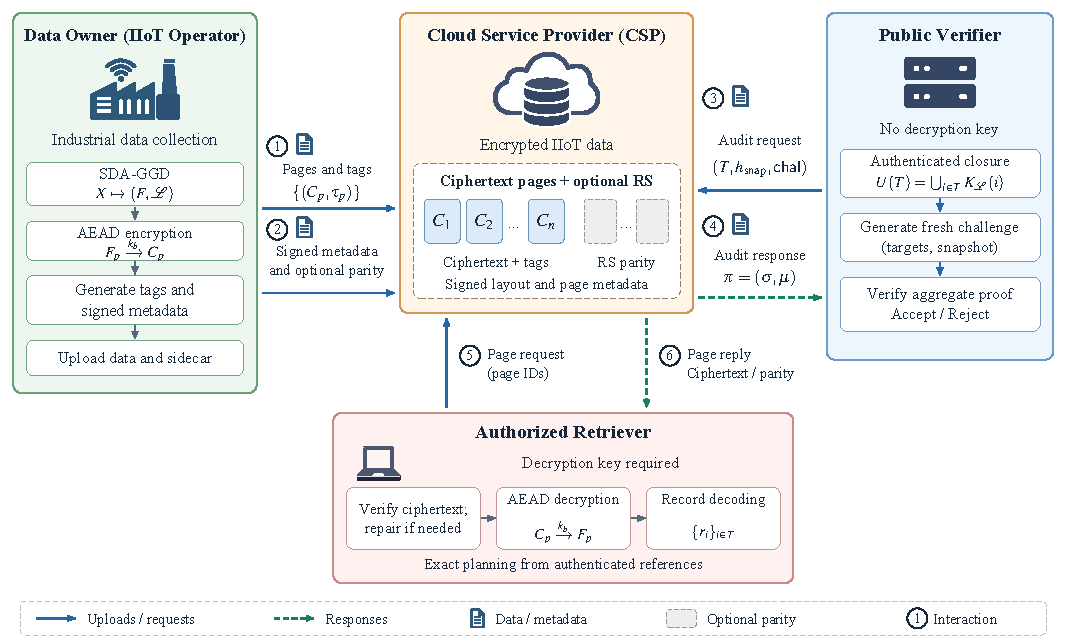
\includegraphics[width=\textwidth]{figures/architecture.pdf}
\caption{System architecture and data flow of ARC-Audit. Public auditing derives
$U(T)$ from the authenticated layout. Authorized recovery authenticates and
decrypts references to determine actual dependencies; original and repaired
ciphertext pass the same checks before decoding. Keyed arrows abbreviate
AEAD sealing/opening under batch key $k_b$, including nonce and associated-data processing.}
\label{fig:architecture}\end{figure*}

\section{ARC-Audit Design}\label{sec:design}
\subsection{Overview}
ARC-Audit connects object selection, response authentication, and record
reconstruction through an authenticated dependency layout
(Fig.~\ref{fig:architecture}). Construction groups and encodes records,
encrypts addressable pages, and authenticates their layout. Public dependency
planning selects and combines the objects needed for sufficient coverage;
aggregate auditing authenticates their linear response to a fresh challenge.
Authorized recovery discovers actual dependencies from authenticated
references and returns records after input verification and complete decoding.

The protection layer supplies authenticated repairs for objects required by
recovery through the same verified access interface. The following subsections
specify these operations and their resource accounting.

\subsection{Cost-Confirmed Shared Representation}\label{sec:c1}
Field grouping must reduce encoded size while preserving the locations
needed for dependency planning. We denote the field-grouped GD construction
by SDA-GGD: sampled gains order candidate merges, and full-input serialized
cost determines acceptance. The resulting layout exposes record spans and
dictionary ranges so that the verifier can select pages before reading references.

\emph{Encoding and serialized cost.}
An exact decimal scale and integer width are declared for each field.
Constants are stored once; remaining fields are partitioned into groups.
For a group $G$ of total width $L_g$, choose $k$ base-bit positions and let
$M_g$ be the number of distinct observed bases. The other $L_g-k$ positions
form the deviation. Each record stores a fixed-width base identifier of
$b_g=\lceil\log_2 M_g\rceil$ bits and its deviation; a dictionary stores the bases.

For $n$ records the serialized group cost is
\begin{equation}\label{eq:cost}
\begin{split}
C(G)={}&C_{\mathrm{hdr}}(G,k)+\lceil M_gk/8\rceil+\lceil nb_g/8\rceil\\
 &+\lceil n(L_g-k)/8\rceil,
\end{split}
\end{equation}
where $C_{\mathrm{hdr}}(G,k)=11+2|G|+2k$ bytes stores the group mode,
field identifiers, and base-bit positions. A RAW group costs
$C_{\mathrm{hdr}}(G,0)+\lceil nL_g/8\rceil$. Separate
rounding is needed because streams are serialized separately. The full
container costs $C_0+\sum_G C(G)$, where $C_0$ contains the fixed schema,
constants, time/label representation, and global header.

\emph{Within-group configuration.}
The configurator stably sorts local bit positions by increasing empirical
binary entropy and tests prefixes of length $k=0,1,\ldots,L_g$.
It stops when $M_g=n$. Among feasible candidates it selects
the smallest byte-rounded cost, with the earlier prefix winning ties.
It selects RAW whenever RAW costs no more than that GD candidate.
Merged groups concatenate their field sequences; entropy ties preserve
this local bit order. The tested configuration selects among these candidates by serialized cost.

\emph{Sample ranking and full-data confirmation.}
Initialization uses one active group per nonconstant field. A fixed
sample supplies the joint byte gain
$\widehat\Delta=C_m(G_a)+C_m(G_b)-C_m(G_a\mathbin{\|}G_b)$,
where $C_m$ configures and measures each group on the same sampled rows,
and $\|$ denotes ordered field concatenation. Only positive estimates enter the queue.
Candidates are refreshed before full-input confirmation, and obsolete
versions are discarded.
Before a merge $(G_a,G_b)$, the encoder reconfigures the combined group
on all input records and computes
\begin{equation}
\Delta_{\mathrm{full}}=C(G_a)+C(G_b)-C(G_a\mathbin{\|}G_b).
\end{equation}
Only positive full serialized-byte gain and positive payload gain permit
acceptance. Affected candidates are updated until the queue is exhausted.
RAW fallback is included in the configuration's real byte cost.
Algorithm~\ref{alg:grouping} takes exact records $X$, schema $\Sigma$,
and fixed sample indices $I$. The helper $\operatorname{Config}(X,G)$
selects a group configuration, including RAW fallback.
$C(G;c)$ denotes serialized cost under configuration $c$, and
$C_{\mathrm{pay}}(G;c)$ denotes its byte-rounded payload cost without the
group header. Omitting $c$ refers to the current configuration.
$\operatorname{SampleGain}$ returns the sampled gain and merged
configuration; sample estimates alone cannot authorize a merge.

In Algorithm~\ref{alg:grouping}, $J$ stores rejected versioned pairs,
$d_e$ counts requeues up to $d_{\max}=8$, and $\operatorname{TopGain}$
returns the stored queue-head gain ($-\infty$ when empty). Supplementary
Section~\ref*{supp-sec:configuration} specifies version checks and tie handling.

\begin{algorithm}[t]\centering\normalsize\setcounter{algline}{0}
\caption{Cost-Confirmed Grouping.}\label{alg:grouping}
\begin{tabular}{@{}r@{\enspace} >{\raggedright\arraybackslash}p{.88\columnwidth}@{}}
\multicolumn{2}{@{}p{\columnwidth}@{}}{\textbf{Require:} Records $X$, schema $\Sigma$, sample indices $I$.}\\
\multicolumn{2}{@{}p{\columnwidth}@{}}{\textbf{Ensure:} Logical container $F$ and public geometry $\mathcal L$.}\\
\al & $\mathcal G\gets$ singleton nonconstant-field groups.\\
\al & Configure $\mathcal G$ on $X$ and $X_I$; $J\gets\varnothing$.\\
\al & $Q\gets$ positive sampled-gain pairs; initialize $d_e=0$.\\
\al & \textbf{while} $Q\neq\varnothing$ \textbf{do}\\
\al & \hspace*{1em}$e=(G_a,G_b,\text{versions})\gets\operatorname{PopMax}(Q)$.\\
\al & \hspace*{1em}\textbf{if} $e$ is stale or $e\in J$, \textbf{continue}.\\
\al & \hspace*{1em}$(\widehat\Delta,\widehat c)\gets\operatorname{SampleGain}(X_I,G_a,G_b)$.\\
\al & \hspace*{1em}\textbf{if} $\widehat\Delta\leq0$, add $e$ to $J$; \textbf{continue}.\\
\al & \hspace*{1em}\textbf{if} $\operatorname{TopGain}(Q)>\widehat\Delta$ and $d_e<d_{\max}$ \textbf{then}\\
\al & \hspace*{2em}$d_e\gets d_e+1$; requeue $e$ with $\widehat\Delta$; \textbf{continue}.\\
\al & \hspace*{1em}\textbf{end if}\\
\al & \hspace*{1em}$G_c\gets G_a\mathbin{\|}G_b$; $c\gets\operatorname{Config}(X,G_c)$.\\
\al & \hspace*{1em}$\Delta_{\mathrm{full}}\gets C(G_a)+C(G_b)-C(G_c;c)$.\\
\al & \hspace*{1em}$\Delta_P\gets C_{\mathrm{pay}}(G_a)+C_{\mathrm{pay}}(G_b)-C_{\mathrm{pay}}(G_c;c)$.\\
\al & \hspace*{1em}\textbf{if} $\Delta_{\mathrm{full}}>0$ and $\Delta_P>0$ \textbf{then}\\
\al & \hspace*{2em}Replace $G_a,G_b$ in $\mathcal G$ by $G_c$ with $(c,\widehat c)$.\\
\al & \hspace*{2em}Invalidate old-group entries; queue positive new/live pairs.\\
\al & \hspace*{1em}\textbf{else} add $e$ to $J$.\\
\al & \hspace*{1em}\textbf{end if}\\
\al & \textbf{end while}\\
\al & $(F,\mathcal L)\gets\operatorname{Serialize}(X,\Sigma,\mathcal G)$.\\
\al & \textbf{return} $(F,\mathcal L)$.\\\bottomrule
\end{tabular}
\end{algorithm}

\begin{proposition}{Confirmed logical cost reduction}\label{prop:cost}
Every accepted merge strictly decreases both the checked logical serialized
cost and its payload cost. Starting from $g_0$ active groups, at most
$g_0-1$ merges are accepted.
\end{proposition}
\begin{claimproof}
Algorithm~\ref{alg:grouping} accepts only positive full-input serialized
and payload gains. Unchanged groups retain their contributions and the
fixed container component is unchanged. Each accepted merge replaces two
groups with one. Rejected versioned pairs are recorded, obsolete entries
are discarded, and bounded requeue counts ensure termination between merges.
\end{claimproof}
The measured secure cost in Eq.~\eqref{eq:cloud-cost} additionally includes
encryption framing, tags and the public manifest. RQ1 evaluates that final
cost separately from the grouping objective.


\subsection{Page Encryption and Authenticated Layout}\label{sec:seal}
Page encryption separates the information needed to locate dependencies
from the values needed to decode them. The public layout contains stream positions, widths, modes, base-bit
positions, dictionary cardinalities, and record counts. The complete logical
container holds the private decoding header and values together with encoded
records. The geometry supports Eq.~\eqref{eq:phi}; numeric constants and
private field values remain in encrypted slices.

For each construction the owner samples a fresh 256-bit batch identifier
$b$ and a random encryption master secret. HKDF-SHA256 derives $k_b$ with
salt $b$ and context \texttt{ARC/ENC/v1}~\cite{RFC5869}.
The nonce is the 96-bit encoding of the local page index. Consequently,
page nonces are distinct under the batch key. AES-256-GCM seals each slice
using Eq.~\eqref{eq:cipher}~\cite{RFC5116}. Associated data is the canonical
encoding of protocol, owner domain, batch, object identity, codec, and
plaintext length. These fields are retained in the public descriptor.

The descriptor additionally records the complete ciphertext length and
hash. Audit tag identity binds this descriptor and the public-parameter
fingerprint. After creating ciphertext objects and tags, the owner signs a
canonical manifest containing their descriptors, public layout, parameters,
and tag-file digest with Ed25519. The manifest digest and signing public
key form the provisioned pins. This order binds tags to immutable objects
and the manifest to completed tags without a circular digest dependency.
Algorithm~\ref{alg:seal} summarizes this construction.

\begin{algorithm}[t]\centering\normalsize\setcounter{algline}{0}
\caption{Seal a Data Batch.}\label{alg:seal}
\begin{tabular}{@{}r@{\enspace} >{\raggedright\arraybackslash}p{.88\columnwidth}@{}}
\multicolumn{2}{@{}p{\columnwidth}@{}}{\textbf{Require:} Logical container $F$, public geometry $\mathcal L$, owner domain.}\\
\multicolumn{2}{@{}p{\columnwidth}@{}}{\textbf{Ensure:} Ciphertext objects, audit tags, signed manifest, and client pins.}\\
\al & Sample fresh batch $b$ and encryption master secret; derive $k_b$.\\
\al & Generate independent audit secret $x$, public parameters $\mathsf{pp}$, and a manifest signing key.\\
\al & \textbf{for each} slice $F_p$ of at most 4068 B \textbf{do}\\
\al & \hspace*{1em}$N_p\gets\operatorname{Encode}_{96}(p)$; form authenticated header $A_p$.\\
\al & \hspace*{1em}$C_p\gets N_p\|\mathsf{Enc}_{k_b}(N_p,F_p,A_p)$.\\
\al & \hspace*{1em}$d_p\gets(A_p,|C_p|,\mathsf{Hash}(C_p))$.\\
\al & \hspace*{1em}$\tau_p\gets\operatorname{Tag}(x,\mathsf{pp},d_p,C_p)$.\\
\al & \textbf{end for}\\
\al & $M\gets\operatorname{Manifest}(b,\mathcal L,\{d_p\},\mathsf{pp},\mathsf{Hash}(\{\tau_p\}))$.\\
\al & Sign canonical $M$; provision signing public key and $\mathsf{Hash}(M)$ as pins.\\
\al & Retain batch-scoped private encoding state and decryption capability.\\
\al & \textbf{return} $\{C_p\},\{\tau_p\},M$, signature, and pins.\\\bottomrule
\end{tabular}\end{algorithm}

\subsection{Authenticated Recovery Closure}\label{sec:c2}
Given targets $T$ and authenticated geometry, public planning returns the
object union $U(T)$. It covers unknown references by including each relevant
group dictionary, yielding sufficient coverage from the geometry alone. Let $S$ cover private structural metadata, $R_g(i)$ the reference span of
record $i$ in group $g$, $V_g(i)$ its deviation or RAW content, and $L(i)$
its labels, all mapped by $\Phi_{\mathcal L}$. Let $\mathcal P_g^{\rm dict}$
contain all mapped dictionary pages for a GD group. Define
\begin{equation}\label{eq:closure}
K(i)=S\cup L(i)\cup\bigcup_g
\bigl(R_g(i)\cup V_g(i)\cup\mathcal P_g^{\rm dict}\bigr).
\end{equation}
For RAW groups the reference and dictionary terms are empty. Private
structure includes the schema and framing needed by the decoder. Label
coverage selects the target's label bits. Every span includes all intersected
ciphertext objects, even when their contents mix several logical streams.

The verifier constructs $K(i)$ using public geometry. Including each
complete group dictionary covers the row selected by any valid BaseID.
The authorized alternative authenticates and decrypts $S$ and the reference
pages, reads each BaseID at its committed position, checks its range, and
maps the referenced dictionary row. Together with $S$, references, local
content, and labels, these rows form $\mathcal D(i)$.

Public requests merge overlaps as $U(T)=\bigcup_{i\in T}K(i)$.
For ciphertext lengths $\ell(p)$, the logical bytes read by an object union
and separate uncached closures are
\begin{equation}\label{eq:reads}
B_U=\sum_{p\in U(T)}\ell(p),\qquad
B_N=\sum_{i\in T}\sum_{p\in K(i)}\ell(p).
\end{equation}
A request cache can also reduce separate traversal to the unique object set.
We distinguish this read-reuse effect from proof aggregation in the controls.
For multiple data batches, targets and unions are computed separately using
batch-qualified identities, then combined at the request level.

\subsection{Fresh Public Aggregate Audit}\label{sec:audit}
The aggregate audit authenticates a linear response over the closure chosen
by the verifier. Binding the targets, snapshot, and selected objects to a
fresh challenge connects the response to the requested records and version.

Every complete ciphertext object is encoded in $s=133$ little-endian sectors
of 31 B, with virtual zero padding. Sector integers satisfy $m_{p,j}<2^{248}<q$
for the BLS12-381 scalar order $q$. Thus the nonce, encrypted payload, and
AEAD tag are all covered; the signed valid length determines tail removal.

The owner selects secret $x$, publishes $Y=xg_2$, and computes tags in
$\mathbb G_1$, with pairing $e:\mathbb G_1\times\mathbb G_2\to\mathbb G_T$:
\begin{equation}\label{eq:tag}
\tau_p=x\left(H(W_p)+\sum_{j=1}^{s}m_{p,j}u_j\right).
\end{equation}
$W_p$ binds the complete ciphertext descriptor and parameter fingerprint.
The bases $u_j$ and descriptor hash $H$ use domain-separated hash-to-curve
operations~\cite{RFC9380}. The construction follows the linear public
authentication structure of Shacham--Waters~\cite{ShachamWaters2013}.

For each batch request, the verifier generates a fresh 256-bit nonce.
The canonical challenge binds the snapshot, parameters, targets, page set,
request policy, and session. Nonzero coefficients $\nu_p$ are derived from
this complete context by hashing its canonical encoding together with the
page index and a retry counter; scalar reduction and zero rejection produce
$\nu_p\in\mathbb F_q^*$. Supplementary Section~\ref*{supp-sec:backend-interface}
specifies the domains and encoding. The CSP returns
\begin{equation}\label{eq:aggregate}
\sigma=\sum_{p\in U}\nu_p\tau_p,\qquad
\mu_j=\sum_{p\in U}\nu_pm_{p,j}\pmod q.
\end{equation}
After context, framing, point, subgroup, scalar-range, and dimension checks,
the verifier tests
\begin{equation}\label{eq:pairing}
e(\sigma,g_2)=e\left(\sum_{p\in U}\nu_pH(W_p)+\sum_j\mu_ju_j,Y\right).
\end{equation}
The verifier retains its own expected page set. Public parameters exclude
invalid or identity bases, and responses must satisfy both parsing rules and
Eq.~\eqref{eq:pairing}. Algorithm~\ref{alg:audit} gives the public flow.

\begin{algorithm}[t]\centering\normalsize\setcounter{algline}{0}
\caption{Public Closure Audit.}\label{alg:audit}
\begin{tabular}{@{}r@{\enspace} >{\raggedright\arraybackslash}p{.88\columnwidth}@{}}
\multicolumn{2}{@{}p{\columnwidth}@{}}{\textbf{Require:} Targets $T$, corresponding manifests and pins, public audit parameters.}\\
\multicolumn{2}{@{}p{\columnwidth}@{}}{\textbf{Ensure:} \texttt{ACCEPT} or \texttt{REJECT}.}\\
\al & Verifier partitions $T$ by immutable batch.\\
\al & \textbf{for each} involved batch $b$ \textbf{do}\\
\al & \hspace*{1em}Authenticate its manifest against the pins; validate $T_b$ and parameters.\\
\al & \hspace*{1em}\textbf{if} validation fails, \textbf{return} \texttt{REJECT}.\\
\al & \hspace*{1em}$U_b\gets\operatorname{SortUnique}(\bigcup_{i\in T_b}K_{\mathcal L_b}(i))$.\\
\al & \hspace*{1em}Sample fresh nonce; bind expected snapshot, request, $T_b$, and $U_b$.\\
\al & \hspace*{1em}Derive $\nu_p\in\mathbb F_q^*$; send challenge and retain expected context.\\
\al & \hspace*{1em}CSP reads unique $C_p$, $p\in U_b$, and responds by Eq.~\eqref{eq:aggregate}.\\
\al & \hspace*{1em}Verifier checks framing, context, encodings, and Eq.~\eqref{eq:pairing}.\\
\al & \hspace*{1em}\textbf{if} any check fails, \textbf{return} \texttt{REJECT}.\\
\al & \textbf{end for}\\
\al & \textbf{return} \texttt{ACCEPT}.\\\bottomrule
\end{tabular}\end{algorithm}

The aggregate occupies 4310 B per batch for this fixed sectorization.
Consequently a request involving $b_T$ batches has $4310b_T$ proof bytes,
in addition to declarations and challenges. Section~\ref{sec:eval} compares
this public interface with authorized reference discovery and public download
using their actual application framing.

For a fixed challenge, the individual-proof control returns
$(\nu_p\tau_p,(\nu_pm_{p,j})_j)$ for each $p$ and verifies the corresponding
single-page equation. Aggregate and individual responses therefore use the
same selected pages and fresh coefficients. Supplementary
Section~\ref*{supp-sec:wire-format} details the serialization.

\subsection{Authenticated Exact Record Recovery}\label{sec:c3}
Exact recovery uses two authenticated stages: discover the references that
identify dependencies, then obtain those dependencies for complete decoding.
The retriever validates the manifest, version pins, and any sidecar binding.
It acquires the structural and reference ciphertext needed to resolve the
targets, checks each object's
identity, length and committed digest, and applies AEAD authenticated
decryption. Only then can it parse the private structure and BaseIDs to
construct exact dependencies. Remaining dictionary rows, deviations, RAW
content and target labels are fetched through the same verified path.

A request-local cache retains authenticated content. The private decoder's
framing is checked against the authenticated public geometry; every bit read
must be present in verified plaintext. After all required inputs are
available, the deterministic decoder reconstructs every requested canonical
record. Authentication, reference-range, framing, or decoding failure yields
$\bot$. Algorithm~\ref{alg:recovery} operates on one batch; multi-batch recovery
applies the same procedure to each involved batch.

Given an object identity and the authenticated batch context, the helper
$\operatorname{VerifiedOpen}$ obtains the committed ciphertext directly or
through the protected fetch interface, verifies its descriptor, and performs
authenticated decryption. It returns the verified plaintext or $\bot$ and
caches only verified ciphertext and authenticated plaintext.

\begin{algorithm}[t]\centering\normalsize\setcounter{algline}{0}
\caption{Authenticated Exact Record Recovery.}\label{alg:recovery}
\begin{tabular}{@{}r@{\enspace} >{\raggedright\arraybackslash}p{.88\columnwidth}@{}}
\multicolumn{2}{@{}p{\columnwidth}@{}}{\textbf{Require:} Manifest and pins, decryption capability, targets $T$, cloud fetch interface, optional signed sidecar.}\\
\multicolumn{2}{@{}p{\columnwidth}@{}}{\textbf{Ensure:} Complete records $\{r_i\}_{i\in T}$ or $\bot$.}\\
\al & Authenticate manifest and sidecar; validate targets and binding.\\
\al & \textbf{if} validation fails, \textbf{return} $\bot$.\\
\al & $I\gets S\cup\bigcup_{i\in T,g}R_g(i)$; $\mathcal C\gets\varnothing$.\\
\al & \textbf{for each} $p\in I$ \textbf{do}\\
\al & \hspace*{1em}$\mathcal C[p]\gets\operatorname{VerifiedOpen}(p)$; on failure \textbf{return} $\bot$.\\
\al & \textbf{end for}\\
\al & Parse authenticated references; check ranges; derive $D(T)$.\\
\al & \textbf{for each} $p\in D(T)\setminus\operatorname{dom}(\mathcal C)$ \textbf{do}\\
\al & \hspace*{1em}$\mathcal C[p]\gets\operatorname{VerifiedOpen}(p)$; on failure \textbf{return} $\bot$.\\
\al & \textbf{end for}\\
\al & Validate private/public framing; decode complete records from $\mathcal C$.\\
\al & \textbf{if} parsing or decoding fails, \textbf{return} $\bot$.\\
\al & \textbf{return} $\{r_i\}_{i\in T}$.\\\bottomrule
\end{tabular}\end{algorithm}

The Conservative control
replaces $I$ in line 3 by $U(T)$; subsequent authentication and decoding are
identical. Exact recovery can thus proceed when an unused dictionary object
is unavailable, provided its actual decoding inputs are available or repairable.

\subsection{Budgeted Ciphertext Protection}\label{sec:protection}
A shared page can be required by several records, so protection allocation
affects which decoding paths remain available. ARC-Audit repairs selected
ciphertext objects within a common storage cap and verifies every repair
before decoding.

A systematic RS$(10,8)$ sidecar over GF$(256)$ groups eight ciphertext
objects and stores two parity shards per stripe. Originals remain in place.
Short objects are virtually padded to 4096 B; incomplete stripes use declared
virtual zero slots. Parity is computed over ciphertext, including nonce and
AEAD tag bytes. A signed sidecar binds the parent snapshot, code dimensions,
stripe members, and parity digests.

Dictionary orders dictionary-containing pages before other objects. Uniform
uses a seeded permutation. FrequencyD ranks objects by dependency frequency
in a reference set of records. The three orders admit a common stripe count
chosen so that every resulting sidecar fits the same per-batch cap:
\begin{equation}\label{eq:budget}
B_{\rm side,b}\leq\left\lfloor\beta B_{\rm cipher,b}\right\rfloor.
\end{equation}
The budget determines how many ciphertext stripes receive protection;
RS$(10,8)$ specifies the redundancy within each admitted stripe.
The charged sidecar contains parity, serialized manifest, signature, signing
public key and digest pin. The evaluation uses $\beta=0.10$ and a NoEC
zero-redundancy reference. Common stripe count and cap hold while actual
serialized sidecar lengths may differ.

Protected retrieval first checks the original. If it is unavailable, the
retriever collects distinct authentic surviving original/parity slots from
its stripe. Eight valid slots permit RS reconstruction. Every reconstructed
real object is truncated to its signed length and checked against its
original ciphertext digest before entering the cache. AEAD authentication
then precedes record decoding. The same helper handles repairs needed by
either the reference-discovery stage or the final exact dependency set.

\subsection{Computation and Storage Accounting}\label{sec:accounting}
Let $N$ be the number of ciphertext objects and $u=|U(T)|$ within a batch.
Direct closure enumeration takes expected
$O(\sum_{i\in T}|K(i)|)$ set-insertion work and $O(u)$ unique-object state,
in addition to resident authenticated metadata. Grouping cost sums the
sample configurations, full-input configurations, and queue updates actually
performed. Each accepted merge decreases the active-group count.

Tag generation processes $Ns$ sectors. A proof accumulates $us$ field
products and $u$ weighted tags; verification forms $u$ descriptor-hash terms
and $s$ sector-base terms, followed by two pairings. Request-level costs sum
across involved batches. Fixed per-batch proof size coexists with page-set
challenge material and a manifest that grows with $N$.

For encoded data without the protection sidecar, secure cloud bytes are
\begin{equation}\label{eq:cloud-cost}
B_{\rm cloud}=B_{\rm cipher}+B_{\rm tags}+B_{\rm manifest},
\end{equation}
where $B_{\rm tags}=48N$ and the signed manifest contains public parameters.
AEAD contributes $28N$ bytes within $B_{\rm cipher}$. Owner-side base bytes
and total private state are separate. A deployed sidecar adds its cloud
files; the accounted protection state also charges its provisioned pins.
This distinguishes stored cloud bytes from client provisioning.

Application traffic includes declarations, challenges, first-stage material
when used, and responses. Initialization authenticates and parses the
manifest and parameters; request timing measures the configured operation
using that context. Recovery timing covers fetching/repair, authentication,
decryption and decoding. Server reads and application replies are separately
accounted, since repair may read several shards to produce one returned page.

\section{Security and Recoverability Analysis}\label{sec:security}
The analysis first establishes exact representation, sufficient dependency
coverage, and binding to authenticated objects. It then treats content
confidentiality, aggregate audit responses, and returned-record authenticity.
The final recovery condition connects these guarantees to available originals
and repair shards. The grouping cost property is established in
Proposition~\ref{prop:cost}.

We assume honest
construction, exact schema arithmetic, valid group configurations, authentic
client pins, and correct provisioned decryption capabilities. Cryptographic
premises are signature unforgeability, collision-resistant hashing, secure
key derivation, nonce-respecting AEAD security, and the selected-set response-authentication
assumption stated below. Table~\ref{tab:security} summarizes their roles.

\begin{table}[t]\centering\small
\caption{Security Properties and Assumptions}\label{tab:security}
\begin{tabular}{@{}>{\raggedright\arraybackslash}p{.39\columnwidth}>{\raggedright\arraybackslash}p{.55\columnwidth}@{}}\toprule
Property & Main premise\\\midrule
Exact representation & Valid schema, complementary bit partition, decoder correctness\\
Content confidentiality & Equal public view, secure derivation, unique nonces, AEAD confidentiality\\
Sufficient closure & Authenticated geometry and complete bit-span mapping\\
Dependency binding & Manifest signature, pinned digest, object-hash binding\\
Selected-set response authentication & Response-authentication assumption for the compact interface\\
Authentic returned records & Bound ciphertext, authenticated decryption, exact decoding\\
Conditional recovery & Required originals or sufficient authentic repair slots\\
Protection cap & Complete serialized-sidecar admission\\\bottomrule
\end{tabular}\end{table}

\subsection{Representation Correctness}\label{sec:representation-proof}
Exact reconstruction follows from the complementary positions of base and
deviation bits. For a configured field group, let $I_g$ contain the chosen base-bit positions
and $J_g$ their complement. A record's group bit string satisfies
$x_{i,g}[I_g]=B_{g,\mathrm{ID}_{i,g}}$ and
$x_{i,g}[J_g]=d_{i,g}$. The stored identifier chooses the exact dictionary
row. Reinserting its bits and the deviation at complementary positions
reconstructs $x_{i,g}$. Inverting the declared widths and exact decimal
scales reconstructs field values; RAW, constants, time and labels follow
their declared representations.

\begin{proposition}{Exact representation}\label{prop:representation}
For an honestly configured batch, authenticated decryption and decoding of
its undamaged required ciphertext objects return the complete canonical records.
\end{proposition}
\begin{claimproof}
AEAD correctness returns the original slices under the bound nonce and
associated data. Their logical positions reassemble the decoder inputs.
Complementary bit reconstruction gives each nonconstant field group, while
RAW and metadata decoding supply the remaining values. Complete field
coverage then yields every canonical record component.
\end{claimproof}

\subsection{Closure Sufficiency and Shared-Object Reuse}\label{sec:closure-proof}
The public closure must cover every object selected by an actual reference.
The following inclusion connects public planning to the decoder inputs.
\begin{proposition}{Sufficient ciphertext coverage}\label{prop:closure}
For every valid target, $\mathcal D(i)\subseteq K(i)$; therefore
$D(T)\subseteq U(T)$ for any valid target set $T$.
\end{proposition}
\begin{claimproof}
Both sets include required structure, references, local content and labels.
For a GD group the exact path selects one valid dictionary row; all objects
intersecting that row belong to the mapped complete dictionary range in
$K(i)$. RAW groups add no dictionary dependency. The map in
Eq.~\eqref{eq:phi} includes every object intersecting a logical bit interval.
Taking unions over groups and targets preserves inclusion.
\end{claimproof}

Let $a_p=|\{i\in T:p\in K(i)\}|$. Then
\begin{equation}\label{eq:reuse}
B_N-B_U=\sum_{p\in U(T)}(a_p-1)\ell(p)\geq0.
\end{equation}
This identity attributes saved uncached reads to overlap. It also explains
why separate traversal with a complete request cache can match union reads.
Aggregation reduces response multiplicity for the chosen set, a distinct
mechanism evaluated with the same challenge and pages.

\subsection{Authenticated Dependency Binding}\label{sec:binding}
The manifest signature and pinned digest authenticate the expected geometry
and ciphertext descriptors. Public selection therefore follows the owner's
committed map. Exact selection additionally authenticates ciphertext
reference bytes, decrypts them under the bound batch key and associated
data, and checks each BaseID before calculating its dictionary row.
Private/public framing consistency checks align this interpretation with
the geometry used to fetch the objects.

Define $\mathsf{BadBind}$ as accepting metadata or an object descriptor
inconsistent with the intended signed snapshot, and $\mathsf{BadHash}$ as
accepting different bytes for a committed ciphertext or parity digest.
Signature unforgeability and collision resistance bound these events under
authentic pins. Conditioned on their absence, substituting a different
reference, page, snapshot or stripe cannot change an accepted decoding input.
The original ciphertext digest is checked after RS reconstruction as well
as on direct retrieval.

\subsection{Content Confidentiality under the Public View}\label{sec:confidentiality}
Confidentiality concerns the encrypted content given the layout and access
information visible to a public observer. Let $\mathsf{Leak}(X)$ specify public batch sizes, object lengths, layout
geometry, group/bit positions, dictionary cardinalities, and the target/access
transcript. Compare two canonical inputs whose public views agree, including
the schedule of selected objects. Encryption keys are independent of data
and separate from signing and audit secrets. Every page nonce is unique
under its batch key.

\begin{proposition}{Confidentiality of private content}\label{prop:confidentiality}
Under secure batch-key derivation and nonce-respecting AEAD confidentiality,
the publicly stored data and public audit views of two equal-leakage inputs are
computationally indistinguishable.
\end{proposition}
\begin{claimproof}
First replace derived batch keys by independent pseudorandom keys under
the key-derivation assumption. For each batch, apply the multi-message
AEAD confidentiality experiment to the equal-length slices with identical
public associated-data fields and distinct nonces. The resulting ciphertext
views are indistinguishable. Descriptors contain public headers, lengths,
and ciphertext hashes. Audit tags, signed manifests, ciphertext parity,
and public audit responses are efficiently generated from that view and
independent authentication secrets. A simulator can generate these objects
and adaptive public responses from the ciphertext view. Such processing
preserves indistinguishability for the stipulated public transcript.
\end{claimproof}
The equal-view condition places geometry and access disclosures directly in
the security definition. Authorized decryption is assigned to a separate role.

\subsection{Audit Correctness and Selected-Set Authentication}\label{sec:audit-scope}
We first establish correctness of the aggregate verification equation, then
state the response-authentication premise used to compose it with closure
selection. The 133 sectors encode up to 4123 B, covering the complete at-most-4096-byte
ciphertext object with prescribed padding. Since each sector integer is
below $q$, sectorization is injective for a fixed valid length. Substitution
of Eqs.~\eqref{eq:tag} and~\eqref{eq:aggregate} yields
\begin{equation}\label{eq:honest}
\sigma=x\left(\sum_{p\in U}\nu_pH(W_p)+
\sum_{j=1}^{s}\left(\sum_{p\in U}\nu_pm_{p,j}\right)u_j\right).
\end{equation}
Bilinearity gives Eq.~\eqref{eq:pairing}, establishing honest correctness.
Response authentication for adaptive challenges is supplied by the following
interface assumption; Proposition~\ref{prop:audit} composes it with the
verifier's authenticated dependency selection.

\emph{Selected-set response-authentication assumption.}
For the instantiated parameters, compact coefficient derivation and validated
adaptive request interface, assume that an adversary has negligible
probability of producing an accepted sector-response vector inconsistent
with the committed ciphertexts for the verifier's challenge. Formally, its
bad event is
\begin{equation}\label{eq:bad-audit}
\mathsf{BadAudit}=\left\{\mathsf{Verify}=1\ \land\
\boldsymbol\mu\neq\sum_{p\in U}\nu_p\mathbf m_p\right\}.
\end{equation}
The interface includes authenticated parameter generation, domain separation,
full challenge-context binding, multiple requests, nonzero coefficient
derivation and canonical response parsing. Supplementary
Section~\ref*{supp-sec:backend-interface} specifies these interfaces.

\begin{proposition}{Conditional closure response authentication}\label{prop:audit}
Under authenticated metadata and the selected-set response-authentication assumption,
an accepted audit authenticates the declared linear response for the
verifier-derived ciphertext closure.
\end{proposition}
\begin{claimproof}
The verifier determines the expected $U(T)$ from authenticated geometry
and retains the bound challenge context. With binding events excluded,
an accepted inconsistent response for that closure is exactly an instance
of $\mathsf{BadAudit}$. The premise applies to each involved batch; a union bound over their bad
events covers the request's batch responses.
\end{claimproof}
This composition gives the audit its specified response meaning. The concrete
retrieval path below authenticates returned page bytes directly.

\subsection{Authenticity of Returned Records}\label{sec:conditional}
Returned-record authenticity follows from binding every decoding input to
the intended ciphertext, including objects reconstructed by repair.
Let $\mathsf{Wrong}$ denote returning a requested record unequal to its
canonical value in the honestly encoded data. Probabilities range over
setup, protocol randomness and the adversary's actions under authentic pins
and correct provisioned keys.

\begin{proposition}{Returned-record authenticity}\label{prop:record-auth}
Under the functional premises, $\mathsf{Wrong}$ implies
$\mathsf{BadBind}$ or $\mathsf{BadHash}$, and hence
\begin{equation}\label{eq:record-auth}
\Pr[\mathsf{Wrong}]\leq\Pr[\mathsf{BadBind}]+\Pr[\mathsf{BadHash}].
\end{equation}
\end{proposition}
\begin{claimproof}
If neither event occurs, every direct or repaired ciphertext used by the
retriever equals its committed object. Authenticated decryption under the
correct key and bound associated data returns its original plaintext.
The authenticated reference positions yield the original BaseIDs, and exact
planning obtains all required decoder inputs. Framing checks and complete
record decoding then return the canonical record by
Proposition~\ref{prop:representation}. Thus an incorrect returned value
requires at least one of the stated binding events.
\end{claimproof}
Direct retrieval and repair therefore establish the same input invariant:
every decoded page matches its committed ciphertext. The bound above uses
that invariant together with decryption and decoder correctness. Since the
signed digest check already fixes the complete ciphertext bytes, this argument
reduces an incorrect returned value to binding failure. AEAD additionally
provides content confidentiality and authenticated opening under the bound key
and associated data. A failed required
check terminates recovery before any partial record is released.

\subsection{Recovery Conditions and Protection Budget}\label{sec:recovery-condition}
Recovery succeeds when all actual dependencies can be obtained through
verified originals or repairs. Let $\mathcal A_0$ be authentic available original ciphertexts,
$\mathcal P_{\rm prot}$ the protected objects, $S(p)$ the ten distinct stripe
slots protecting $p$, and $\mathcal V$ the authentic available slots,
including prescribed virtual zeros.
\begin{proposition}{Sufficient exact recovery condition}\label{prop:recovery}
With authentic metadata and correct decryption capability, Exact recovery
succeeds if
\begin{equation}\label{eq:recovery-condition}
\forall p\in D(T):\quad p\in\mathcal A_0\ \lor\
\bigl[p\in\mathcal P_{\rm prot}\land|S(p)\cap\mathcal V|\geq8\bigr].
\end{equation}
\end{proposition}
\begin{claimproof}
Each required object is either directly authenticated or reconstructed from
eight distinct authentic slots and checked against its original commitment.
The initial structure/reference objects are part of $D(T)$, so the same
condition supports dependency discovery. The remaining actual objects can
then be acquired, authenticated and decoded. Proposition~\ref{prop:representation}
completes the argument.
\end{claimproof}
Conservative recovery applies the corresponding condition to $U(T)$.
Since $D(T)\subseteq U(T)$, exact selection avoids availability requirements
for unused dictionary objects. The sufficient condition concerns available
slots, irrespective of the particular erasure distribution.

Finally, admission computes the complete serialized sidecar cost and accepts
a common stripe count only when all protected orders satisfy
Eq.~\eqref{eq:budget}. This enforces the declared cap over parity and
associated authentication state. The experiments compare the resulting
allocation choices using the same budget and code.

\section{Experimental Evaluation}\label{sec:eval}
The evaluation follows the three design contributions. RQ1 measures the
storage and construction costs of the shared representation. RQ2 measures
the communication and computation of public dependency planning and aggregate
auditing. RQ3 examines how protection allocation and dependency selection
affect authenticated record recovery. Table~\ref{tab:scope} records the workload
size and experimental unit of each comparison.

\begin{figure*}[t]\centering
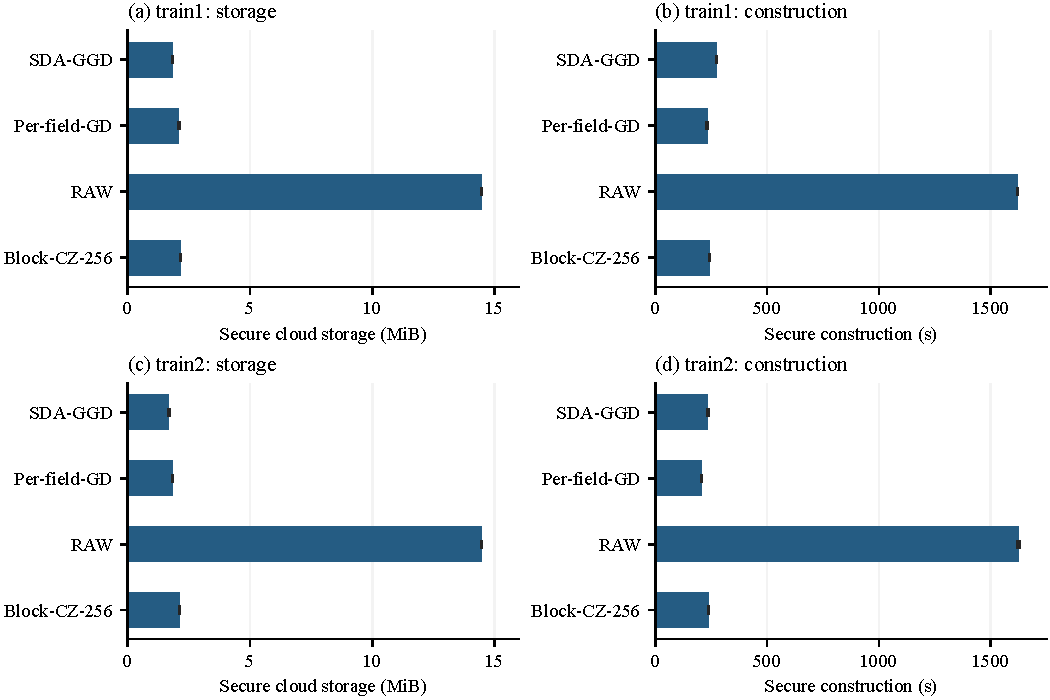
\includegraphics[width=\textwidth]{evidence/current-secure/figures/c1.pdf}
\caption{Secure cloud storage and complete construction time for the two
21,600-record C1 windows. Bars show medians of two builds; whiskers show
observed minima and maxima. Cloud storage includes ciphertext, audit tags
and the signed public manifest.}
\label{fig:key-c1}\end{figure*}
\begin{figure*}[t]\centering
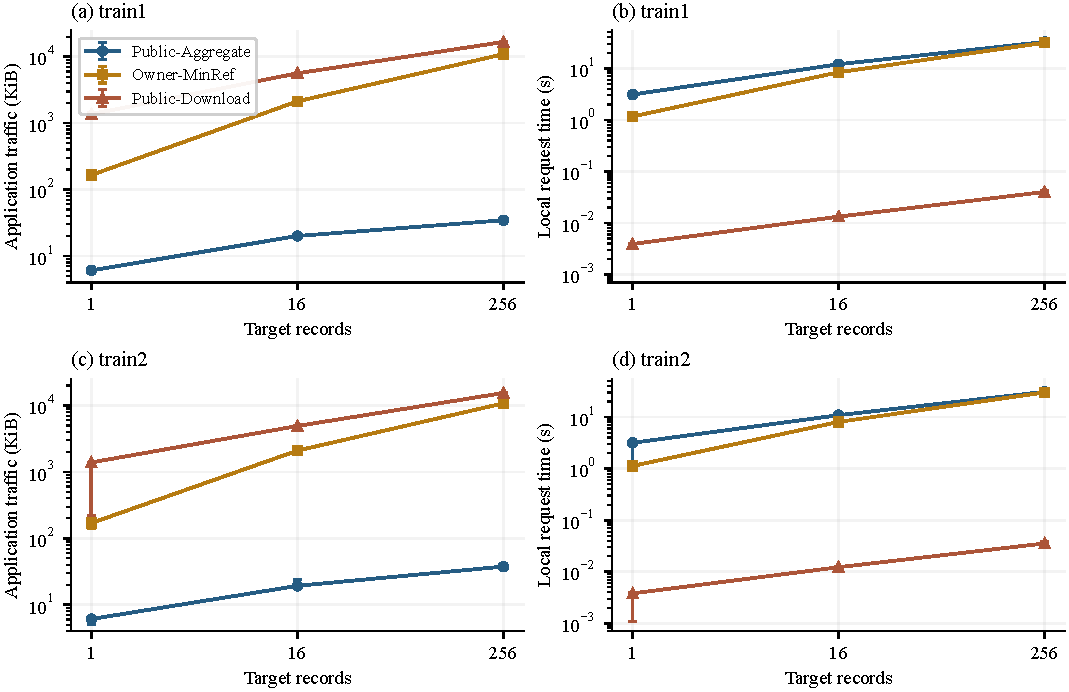
\includegraphics[width=\textwidth]{evidence/current-secure/figures/c2.pdf}
\caption{C2 application traffic and complete local request time on the full
train1/train2 workloads. Points show medians of three matched target sets per
method and target count; whiskers show observed ranges. Owner-MinRef has
authorized decryption capability. Initialization is accounted separately.}
\label{fig:key-c2}\end{figure*}
\begin{figure*}[t]\centering
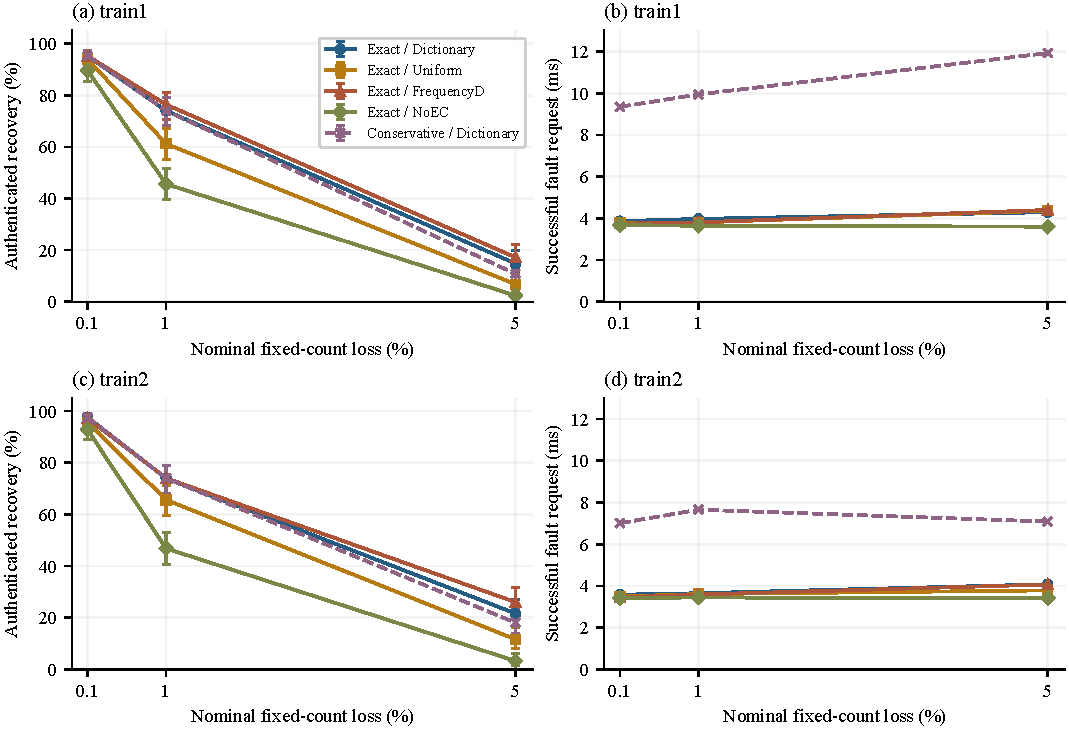
\includegraphics[width=\textwidth]{evidence/current-secure/figures/c3.pdf}
\caption{C3 authenticated single-record recovery on full train1/train2 workloads.
Success points include 250 cases over five layouts with pointwise 95\% Wilson
intervals. Time points are medians of successful fault requests. Four Exact
allocation policies and Conservative/Dictionary separate placement from
dependency policy. Losses are drawn from the common population of original
objects and deployed parity slots. Protected orders use a common stripe
count; parity and authentication metadata together are capped at 10\% of
batch ciphertext bytes.}
\label{fig:key-c3}\end{figure*}

\subsection{Experimental Setup}
\subsubsection{Data and Implementation}
The source is HAI 21.03 train1 and train2~\cite{Shin2021HAI}, containing
216,001 and 226,801 records. The 84 source columns comprise time, 79 process
fields and four attack indicators. Three process-specific indicators are
encoded independently; the combined indicator is derived from them.
Exact decimal canonicalization preserves process values. After each recovery
operation, an independent scorer checks $\widehat r_i=r_i$ against the canonical
source, separately from the client's authentication and complete-decoding checks.

C1 uses a six-hour window starting at 00:00 on July 11 and August 1,
2020, for train1 and train2, respectively, with 21,600 records per window.
C2 and C3 use all records, partitioned into three data batches for train1
and four for train2. Batch sizes and source identities are given in
Supplementary Section~\ref*{supp-sec:key-evidence}. Each batch is
configured and sealed independently. These are two workloads from one HAI source. Paired values below follow
train1/train2 order.

The implementation uses Python 3.10.12, NumPy 2.2.6, cryptography 50.0.1
and py-ecc 8.0.0. It combines AES-256-GCM, Ed25519, the BLS12-381 full-page
authenticator, and ciphertext RS$(10,8)$. The C1 and full-segment processes
were pinned to separate CPU affinity sets, $\{2\}$ and $\{4\}$, on a shared
host. Input preparation and independent scoring occur outside measured
construction or request operations. Provisioned manifests and verifier
contexts are initialized separately from request timing.

\begin{table}[t]\centering\small
\caption{Evaluation Workloads and Experimental Units}\label{tab:scope}
\begin{tabular}{@{}l>{\raggedright\arraybackslash}p{.31\columnwidth}>{\raggedright\arraybackslash}p{.48\columnwidth}@{}}\toprule
Focus & Records per segment & Comparisons and observations\\\midrule
C1 & 21,600 / 21,600 & 4 methods, 2 builds each; 16 observations\\
C2 & 216,001 / 226,801 & 3 target sizes, 3 cases, 3 interfaces; 54 requests\\
C3 & 216,001 / 226,801 & 5 layouts, 3 loss rates, 50 cases, 8 controls; 12,000 fault outcomes\\
Clean & Same as C3 & 30 cases, 1 layout, 8 controls; 480 outcomes\\\bottomrule
\end{tabular}\end{table}

\subsubsection{Controls and Metrics}
C1 compares SDA-GGD, Per-field-GD, RAW canonical encoding, and Block-CZ-256.
Block-CZ-256 serializes nonconstant columns within blocks of 256 records and
compresses each block as an independent Zstd frame at level 3. Per-field-GD
isolates the grouping choice; RAW and Block-CZ-256 provide alternative
representations. All receive the same secure sealing and accounting. Cloud bytes include ciphertext,
audit tags and the signed public manifest. Owner base bytes and total
private disk state are separate. Construction covers configuration,
encoding and complete secure sealing from normalized input.

The configuration
sample has $\min(50{,}000,n)$ rows, equal to the full 21,600-row C1 window.
This setting evaluates grouping with full-window ranking and full-input
cost confirmation. Each method/window has two runs; plots show the median
and observed range.

C2 distinguishes dependency discovery from the response format. It uses
$r=1,16,256$ targets and three target sets per segment/size. The
Public-Aggregate interface selects the public closure; Owner-MinRef-Aggregate
(shortened to Owner-MinRef in plots and tables) authenticates and decrypts
the reference material needed to identify exact dependencies; Public-Download
returns public-closure ciphertext for hash verification. The public interfaces use no decryption key. The MinRef
control has authorized decryption capability. Public-Aggregate versus Public-Download compares response formats under
the same public access capability. Public-Aggregate versus Owner-MinRef then
compares dependency planning with different access capabilities.

All three share the same
targets within a case. Cross-batch targets are served through their respective
batch contexts. Application bytes include declarations, challenges,
first-stage material and responses. Complete local request time includes
planning and the work executed by the request interface. Initialization
is reported separately; the time axis measures local processing rather
than network transfer. Each point reports a median and min--max range.

C3 combines Exact and Conservative recovery with four allocation controls:
Dictionary, Uniform, FrequencyD, and NoEC. Fixing Exact compares allocation;
fixing a sidecar compares the dependency policy. NoEC supplies the
zero-redundancy reference.

Protected orders share RS$(10,8)$, an admitted stripe count, and a per-batch
10\% ciphertext-byte cap including parity and signed sidecar state.
FrequencyD uses the first $\min(4096,\max(1,n/5))$ reference records of
each batch, with integer division for $n/5$. Recovery targets exclude these
reference ranges. The 7200-record batch has 1440 reference records; the
other six batches each have 4096. The scorer accesses source records only
after the service timer ends; recovery obtains content through the cloud
fetch interface and authenticated repairs.

\subsubsection{Faults and Statistics}
For each segment, five seeded protection layouts are evaluated at nominal
loss fractions $\alpha=0.001,0.01,0.05$, with 50 cases per layout/rate.
Each case selects one target and a fixed-count loss mask without replacement
from the segment-wide union of original objects and deployed parity slots.
The population sizes are $N_{\mathrm{fault}}=5000$ and $4765$, giving $\lceil\alpha N_{\mathrm{fault}}\rceil$
loss counts of 5/50/250 and 5/48/239. A target accesses its own batch
within this population. Controls share targets and slot-loss masks; NoEC
uses the corresponding original-page losses. Policy order is rotated across cases.

Each fault-success point includes all 250 outcomes and a pointwise 95\%
Wilson interval conditional on the five tested layouts. Successful fault
requests supply the recovery-time medians. Their success sets may differ,
so these times are interpreted alongside success probabilities. Clean
recovery uses 30 cases per segment/control on one layout, giving 480
successful complete-record checks. Full eight-control results, failure
timings and initialization measurements appear in the supplement.



\subsection{RQ1: Storage and Secure Construction}
SDA-GGD reduces secure cloud storage relative to Per-field-GD on both
windows (Fig.~\ref{fig:key-c1}). Its stored sizes are 1,903,138 and
1,770,118 B, compared with 2,198,812 and 1,938,839 B for Per-field-GD:
reductions of 13.45\% and 8.70\%. Block-CZ-256 stores 2,278,001 and
2,227,359 B, while RAW stores approximately 15.17 MB per window.
All 16 constructions pass canonical decoding checks. Supplementary
Table~\ref*{supp-tab:key-c1-statistics} provides the byte and timing ledger.

The storage reduction trades additional encoding work against lower tag
generation cost. Complete secure construction takes median times of 274.356/235.621 s for
SDA-GGD and 231.521/206.163 s for Per-field-GD, an increase of
18.50\%/14.29\%. These are descriptive ratios of the observed medians.
SDA-GGD's codec stage takes 73.66/47.63 s, compared with 1.00/0.83 s for
Per-field-GD, reflecting repeated group configuration and full-cost confirmation.
However, fewer resulting objects reduce its tag-generation time to
200.42/187.72 s from 230.25/205.05 s. The complete construction cost
therefore combines more encoding work with less authentication work.

The stored representation and owner-side state account for different
resources (Table~\ref{tab:state}). SDA-GGD retains 303,595/184,687 B of base content within
335,884/215,702 B of total private state. Per-field-GD retains
208,267/174,552 B of bases within 245,064/209,287 B total. On these windows, grouping reduces
secure cloud storage while retaining more owner-side private state than
Per-field-GD. These measurements characterize
the representation and secure construction together.



\begin{table}[t]\centering\small
\caption{C1 Cloud and Owner State}\label{tab:state}
\begin{tabular}{@{}lrrrr@{}}\toprule
& \multicolumn{2}{c}{Cloud (MiB)} & \multicolumn{2}{c}{Owner (KiB)}\\
Method & train1 & train2 & train1 & train2\\\midrule
SDA-GGD & 1.815 & 1.688 & 328.012 & 210.646\\
Per-field-GD & 2.097 & 1.849 & 239.320 & 204.382\\
RAW & 14.463 & 14.463 & 0.227 & 0.227\\
Block-CZ-256 & 2.172 & 2.124 & 0.234 & 0.234\\
\bottomrule\end{tabular}
\tabnote{Medians of two builds per window. Owner state includes the base catalog and private encoding/key files. Protection is accounted separately.}
\end{table}

\subsection{RQ2: Public Audit Communication and Computation}
\emph{Responses under the same public access capability.}
Public-Aggregate and Public-Download use the same public closure but return
an aggregate proof and ciphertext pages, respectively (Fig.~\ref{fig:key-c2}).
At $r=256$, Public-Aggregate transfers 35,405/38,524 B and takes
32.532/30.908 s of local processing. Public-Download transfers
17,041,940/15,754,868 B and takes 0.0400/0.0354 s.
Aggregate authentication reduces response traffic through group and field
arithmetic, whereas downloading permits inexpensive local digest verification.
The measured tradeoff is therefore lower application traffic at higher local
processing cost. These local timings and byte counts describe the two
resources separately; end-to-end time also depends on network transfer.

\emph{Dependency discovery under different access capabilities.}
Public planning obtains sufficient coverage from authenticated geometry.
Owner-MinRef-Aggregate first authenticates and decrypts reference material
to narrow its final dictionary coverage. At $r=256$, its application traffic
is 11,163,473/11,010,612 B and its local processing takes 31.532/30.148 s.
Relative to this authorized interface, Public-Aggregate reduces traffic by
99.68\%/99.65\% while increasing local processing by 3.17\%/2.52\%.
These percentages are ratios of medians, not paired effect intervals.

For a single target, Public-Aggregate takes 3.106/3.169 s, versus
1.164/1.126 s for Owner-MinRef. Public traffic is 6237/6254 B,
versus 169,601/173,696 B. Reference discovery reduces MinRef's final
object coverage, while public planning eliminates the first-stage transfer.
As the target set grows, overlap and the union of references change this
balance. The $r=16$ points show intermediate costs; all per-size values are
in Supplementary Table~\ref*{supp-tab:key-c2-statistics}.

\emph{Traffic composition.}
Application traffic consists of request declarations and challenges,
first-stage material when used, and the final response. At $r=256$, the
median first-stage transfer for Owner-MinRef is 11,128,596/10,972,500 B;
the two public interfaces have no such phase. Both aggregate interfaces
return 12,930/17,240 B of proofs for the three/four involved batches.
Each batch contributes 4310 B for the fixed sector count, while declarations
and challenges depend on the request. Supplementary
Table~\ref*{supp-tab:c2-accounting} separates these components, server reads,
and initialization. For $r=1$, the required contexts have median setup times
of 8.101/7.805 s, separate from the request times above. Each batch context is
initialized once and reused; these values describe the contexts needed by
the requests, rather than a setup charge repeated for every request. All 54
honest requests pass their declared verification interface.

\emph{Mechanism controls.}
Two representative 16-target controls isolate object reuse and aggregation.
On the train1 batch, union reads 805 objects (3,297,280 B), compared with
5643 reads (23,113,728 B) for uncached separate traversal. Separate traversal
with a request cache also reads 805 objects. The analogous train2 control
has 125 versus 892 uncached reads, with both cached strategies reading 125.
This establishes the role of reuse independently of a particular traversal.

For the same selected pages and coefficients, the aggregate proof is 4310 B,
whereas the individual-proof totals are 3,475,990 B and 539,750 B for the
two controls. Verification time decreases from 472.659 to 3.477 s and
from 73.646 to 1.074 s, respectively. These representative controls explain
the mechanism; the repeated request experiment supplies the main traffic
and time curves. Both controls reject the tested last-byte ciphertext
mutation, consistent with the full-frame authentication design.



\subsection{RQ3: Authenticated Recovery and Protection Allocation}
\emph{Protection placement.}
Holding Exact recovery fixed isolates protection allocation. Dictionary
increases recovery success over
Uniform and NoEC under the common cap (Fig.~\ref{fig:key-c3}). At 1\%
nominal loss, Dictionary recovers 185/250 records on each segment (74.0\%),
compared with 153/250 and 164/250 for Uniform (61.2\%/65.6\%). The
observed differences are 12.8/8.4 percentage points. NoEC recovers
114/250 and 117/250 (45.6\%/46.8\%). At 0.1\%, Dictionary reaches
95.2\%/97.6\%, compared with Uniform's 94.0\%/95.6\%.

\emph{Frequency-based allocation.}
At 5\%, FrequencyD with Exact recovery obtains 43/250 and 65/250
successes (17.2\%/26.0\%), compared with Dictionary's 14.8\%/21.6\%.
At 0.1\% the two policies are equal on train1, while Dictionary is slightly
higher on train2. FrequencyD prioritizes frequently used dependency objects
from its reference records; Dictionary prioritizes object type. With the code,
stripe count, and budget held fixed, these differences show how protection
allocation across record dependencies affects recovery success.
Supplementary Table~\ref*{supp-tab:key-c3-statistics} retains all eight controls.

\emph{Dependency policy.}
Holding the Dictionary sidecar fixed isolates the dependencies required for
recovery. Exact and Conservative have the same
success outcomes at 0.1\% and 1\% loss. At 5\%, Exact recovers
37/250 and 54/250 (14.8\%/21.6\%), whereas Conservative recovers
27/250 and 45/250 (10.8\%/18.0\%). Exact gains ten and nine paired
cases, with no reverse loss in these pairs. Removing unused dictionary
requirements matters when such objects are unavailable but the actual
record dependencies remain recoverable. The measured availability benefit
therefore varies with the failure condition and allocation policy.

\emph{Recovery time.}
Clean Dictionary/Exact recovery takes 3.693/3.507 ms, compared with
8.991/7.205 ms for Conservative. With the same successful target population,
exact selection lowers the amount of authenticated content acquired and decoded.
At 5\% loss, successful Dictionary/Exact requests take median times of
4.298/4.074 ms, while Conservative takes 11.933/7.079 ms. These fault
time medians include retrieval and any repair work for successful requests;
the successful populations differ across controls. Reading them with the
success curves distinguishes inexpensive completion from the probability
of obtaining a complete record. Supplementary
Table~\ref*{supp-tab:key-c3-time} reports success counts beside latency,
and the full ledger retains failed-request times.

Taken together, the controls identify two distinct effects. Allocation
protects different shared objects under the same code and cap. Dependency
selection determines which of those objects a requested record actually
requires. Authenticated exact recovery combines the two while preserving
the same ciphertext verification and complete-record acceptance rules.

\section{Conclusion}
ARC-Audit connects public auditing and authenticated record recovery through
an authenticated mapping from industrial IoT records to ciphertext objects.
Public geometry supplies sufficient coverage, while verified private references
identify the actual recovery dependencies. Original and repaired objects follow
the same authentication and complete-decoding rules. The evaluation shows
storage and communication savings with corresponding construction and local
computation costs. It also shows that protection allocation and dependency
selection jointly determine recovery. Exact selection permits complete
record recovery when the authenticated inputs required by the decoder remain
obtainable, even if unused shared objects are unavailable.

\IEEEtriggeratref{24}
\bibliographystyle{IEEEtran}
\bibliography{IEEEabrv,bstcontrol,references}
\end{document}
